\section{Objective and significance of the study}
\label{sec:objective}

\subsection{Objective}

The objective of this study is to detect relations between the issues of a software project and how they
are related. To achieve this goal we try to develop an algorithm which is able to match the descriptions
of issues and the commit messages. To test and improve this algorithm we use the data of an real software
project until it turns out satisfactory. The results of the algorithm are evaluated by ourselves wherefore
a user study is strongly recommended.

\subsection{Significance}
The significance of this study become clear by viewing some scenarios:
Since most software systems consists of thousands lines of code it is really heavy for new new developers
to understand the existing code. There are multiple ways to help these developers to get into the code.
One option is a good documentation of the code. To improve the advantage taken by such a documentation it
should contain multiple diagrams and similar graphics describing the code.

Usually a software project is not documented as good as it should be that new programmers can understand
the existing code with low effort. Some documentations contain only a few graphics if there is a
documentation at all since the creation is very time-consuming. In order to save expenses the creation and
due the fact that the documentation has mostly just secondary importance the developers doesn't invest
enough time to create a proper documentation. Since creating graphics is a very time-consuming task,
especially when they won't be generated, most documentations have a lack of them.

New developers need to get an understanding how application works internally. Therefore they need to know
how the individual parts interact with each other. 
By matching issues with commit-messages new developers can see which changes are made to implement a new
feature by taking a look at the changed files. This is a time-consuming task, too. But the opportunity to
understand which changes are made to the code in order to add new functionality to the applications gives
the possibility to get an understanding how the code is designed. That's why using a software which
matches the issues with the commits allows a deeper understanding of the code.


\begin{figure}[H]
\centering
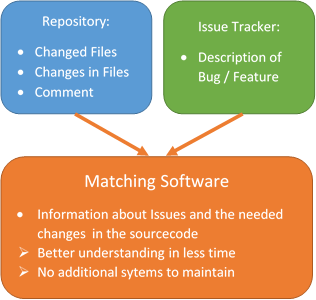
\includegraphics[width=0.5\textwidth]{MatchingUseCase.png}
\caption{Benefits from Matching}
\label{MatchingBenefits}
\end{figure}

The matching of issues and commits is independent of the creation of a documentation, yet it doesn't allow
to refrain it. Since most development teams work with any kind of version management software and a
software to track their bugs and issues they have all they need in order to use such a software as we
describe in this paper. In conclusion the developers don't need to install and maintain additional
software but they have the benefit of the matching. That means that they don't have any effort if they
just create comprehensive commit messages and issues.